% !TEX spellcheck = de_DE
% !TeX root = Vorlesung.tex
%---------------------------------------------------------------------------------
\section[Tragflügeltheorie]{Tragflügeltheorie}\label{sec:AAD}
%---------------------------------------------------------------------------------
\miniframesoff
\begin{frame}<handout:0>[noframenumbering]{Content}
\tableofcontents[currentsection]
\PutAt<1-|handout:0>[5cm]{(10cm,2cm)}{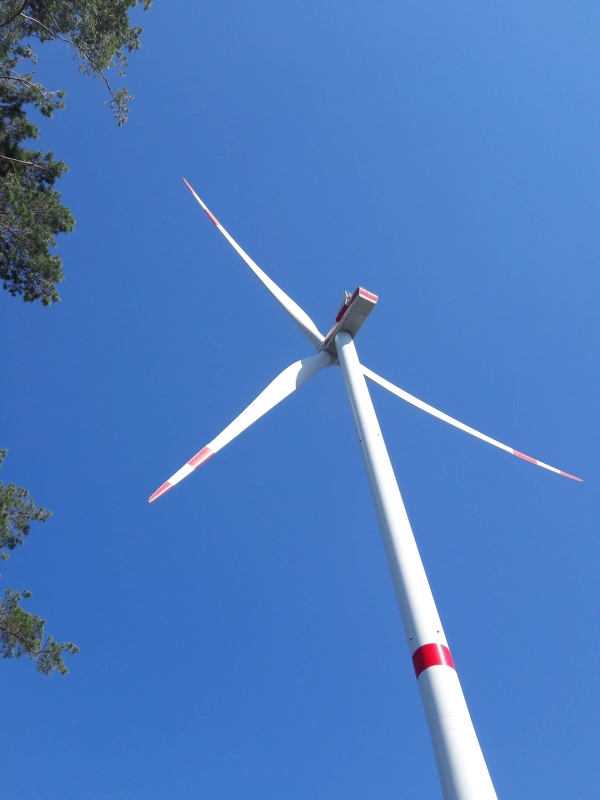
\includegraphics[width=4.0cm]{\StylePath/content/Fronrot}} % graphic related to topic	
\end{frame}
\miniframeson
%---------------------------------------------------------------------------------
\begin{frame}{Tragfügel/Aerodynamisches Profil} 
\begin{columns}
	\column{7cm}
		\centering
		\includegraphics<1->[width=7.0cm] {AAD/Airfoil}\\
		{\tiny\textcolor{gray}{[\href{https://en.wikipedia.org/wiki/Airfoil}{wikipedia}]}}		
	\column{7cm}
		\begin{block}<1->{Definition}
		 	\begin{itemize}
				\item In der Fluiddynamik wird ein Tragflügelprofil als die Form eines Festkörperquerschnitts in Strömungsrichtung bezeichnet.
				\item Aufgrund der spezifischen Form des Tragflügels erzeugt eine Strömung einer Flüssigkeit oder eines Gases äußere Kräfte auf den Körper.
			\end{itemize}						 
		\end{block}
\end{columns} 	
\end{frame}
%---------------------------------------------------------------------------------
\begin{frame}{Vereinfachte physikalische Erklärungen zum Auftrieb 1/3} 
\begin{columns}
	\column{6cm}
		\centering
		\includegraphics<1->[width=6.0cm] {AAD/AirfoilDeflectionLift_W3C}\\
		{\tiny\textcolor{gray}{[\href{https://en.wikipedia.org/wiki/Lift_(force)}{wikipedia}]}}				
	\column{8cm}
		\begin{block}<1->{Strömungsumlenkung und Newtonsche Gesetze}	
		 	\begin{itemize}
				\item Wenn der Luftstrom den Tragflügel passiert, ändert er die Richtung nach unten.
				\item Nach dem 2. Newtonschen Gesetz ($F=ma$) erfordert dies eine nach unten gerichtete Kraft, die vom Tragflügel auf die Luft ausgeübt wird.
				\item Nach dem 3. Newtonschen Gesetz (Aktions-Reaktions-Gesetz) wird durch die Luft eine Reaktionskraft auf den Tragflügel ausgeübt, die diesen nach oben drückt.
			\end{itemize}				
		\end{block}
\end{columns} 	
\end{frame}
%---------------------------------------------------------------------------------
\begin{frame}{Vereinfachte physikalische Erklärungen zum Auftrieb 2/3} 
\begin{columns}
	\column{6cm}
		\centering
%		\includegraphics<1->[width=6.0cm] {AAD/Karman_trefftz.png}\\
		\animategraphics[loop,autoplay,width=6cm]{30}{AAD/Karman_trefftz_gif/Karman_trefftz-}{0}{79}
		{\tiny\textcolor{gray}{[\href{https://en.wikipedia.org/wiki/Lift_(force)}{wikipedia}]}}				
	\column{8.5cm}
		\begin{block}<1->{Erhöhte Strömungsgeschwindigkeit und das Bernoulli-Prinzip}	
			\begin{itemize}
			    \item \small{Die Stromlinien auf der Oberseite des Tragflügels werden komprimiert, wodurch die Strömungsgeschwindigkeit erhöht wird.}
				\item Die Luftgeschwindigkeit auf der Oberseite des Tragflügels ist höher als auf der Unterseite.
				\item Nach Bernoullis Gesetzes verursacht eine erhöhte Geschwindigkeit einen Bereich mit niedrigerem Druck (Saugseite) und eine verringerte Geschwindigkeit einen Bereich mit höherem Druck (Druckseite).
				\item Dieser Druckunterschied erzeugt eine Kraft, die von der Druckseite zur Saugseite des Tragflügels wirkt.
			\end{itemize}			
		\end{block}
\end{columns} 	
\end{frame}
%---------------------------------------------------------------------------------
\begin{frame}{Vereinfachte physikalische Erklärungen zum Auftrieb 3/3} 
\centering
\includegraphics<1->[height=6.5cm] {AAD/UnderstandingAerodynamicLift}\\
{\tiny\textcolor{gray}{[\href{https://www.youtube.com/watch?v=E3i_XHlVCeU}{youtube - The Efficient Engineer}]}}					
\end{frame}
%---------------------------------------------------------------------------------
\begin{frame}{Wie funktionieren Flügel?} 
\begin{columns}
	\column{4.5cm}
	\centering
	\includegraphics<1->[height=7.2cm] {AAD/Babinsky2003_Fig7_to_9}
	\column{9.5cm}
	\begin{block}<1->{Eine weitere Erklärung \cite{Babinsky2003}}	
		\begin{itemize}
			\item \small{Ein Partikel auf einer gekrümmten Stromlinie ändert die Richtung. Daher muss eine Zentripetalkraft vorhanden sein. Diese Beschleunigungskraft wird durch Druckunterschiede (Druckgradient senkrecht zur Stromlinie) erzeugt.}
			\item Der Druck nimmt zum Krümmungszentrum hin ab. In A und C ist der Druck gleich ($p_{\textnormal{A}}=p_{\textnormal{C}}=p_{\textnormal{atm}}$). Wenn man auf einer Linie von A nach B fährt, nimmt der Druck in Richtung B ab ($p_{\textnormal{A}}>p_{\textnormal{B}}$). Wenn man auf einer Linie von C nach D fährt, steigt der Druck in Richtung D. ($p_{\textnormal{C}}<p_{\textnormal{D}}$).
			\item Das bedeutet $p_{\textnormal{B}}<p_{\textnormal{D}}$. Die Druckdifferenz erzeugt einen Auftrieb.
			\item  \href{https://www.cam.ac.uk/research/news/how-wings-really-work}{[Video University of Cambridge]}
		\end{itemize}			
	\end{block}
\end{columns} 			
\end{frame}
%---------------------------------------------------------------------------------
\begin{frame}{Lösung für das Problem} 
\begin{columns}
	\column{8.5cm}
	\centering
	\includegraphics<1->[width=8.5cm] {AAD/Ansys}\\
	{\tiny\textcolor{gray}{[\href{https://www.youtube.com/watch?v=ngNZdyWTUIo}{youtube - ANSYS CFX Tutorial}]}}	
	\column{5.5cm}
	\begin{block}<1->{Komplexere Lösung}	
		Berechnung Auftrieb mit CFD
		\begin{itemize}
			\item Impulserhaltung
			\item Massenerhaltung
			\item Energieerhaltung
		\end{itemize}			
	\end{block}
	\begin{block}<2->{Einfache Lösung}	
		\begin{itemize}
			\item Experten diskutieren immer noch über eine vereinfachte physikalische Erklärung.
			\item Wichtig für uns: Anströmen eines Tragflügels erzeugt Auftrieb und Widerstand!
		\end{itemize}			
	\end{block}
\end{columns} 			
\end{frame}
%---------------------------------------------------------------------------------
\begin{frame}{Auftrieb und Widerstand} 
\setlength{\abovedisplayskip}{0pt}
\setlength{\belowdisplayskip}{1pt}
\begin{columns}	
	\column{7.5cm}
	\begin{block}<1->{Auftriebskraft $L$ und Widerstandskraft $D$}
		\begin{align*}
		L   & = \frac{1}{2} \rho \left(cb\right) c_{\textnormal{L}}(\alpha_{\textnormal{A}}) w^2\\
		D   & = \frac{1}{2} \rho \left(cb\right) c_{\textnormal{D}}(\alpha_{\textnormal{A}}) w^2
		\end{align*}
		\begin{tabular}{ll}
			$c_{\textnormal{L}}$ 		&  	Auftriebsbeiwert\\
			$c_{\textnormal{D}}$ 		&  	Widerstandsbeiwert\\
			$\alpha_{\textnormal{A}}$ 	&  	Anstellwinkel\\
			$c$ 					& 	Profiltiefe \\
			$b$ 					& 	Profilbreite \\
			$w$ 					& 	lokale (relative) Windgeschwindigkeit
		\end{tabular}	
	\end{block}
	\column{7cm}
	\centering
	\includegraphics<1->[width=7.0cm] {AAD/LiftAndDrag.pdf}
	\begin{block}{Per Definition}
		\begin{itemize}
			\item Auftrieb senkrecht zu $w$
			\item Widerstand parallel zu $w$	
		\end{itemize}
	\end{block}
\end{columns} 	
\end{frame}
%---------------------------------------------------------------------------------
\begin{frame}{Beispiel: NACA64 A17 von NREL 5~MW RWT} 
\begin{columns}	
	\column{7cm}
	\centering
	\includegraphics<1->[height=3.5cm] {AAD/NREL5MW}\\
	{\tiny\textcolor{gray}{\cite{Jonkman2009a}}}
	\begin{block}{Referenzwindkraftanlage}
		\begin{itemize}
			\item für Open FAST (Open Source)
			\item \SI{126}{m} Rotordurchmesser
			\item \SI{90}{m} Nabenhöhe
			\item NACA64 für Spitzenbereich	
		\end{itemize}
	\end{block}	
	\column{7cm}
	\includegraphics<2->[width=7.cm] {AAD/NACA64_618}\\
	\includegraphics<2->[width=7.cm] {AAD/NACA64_LiftAndDrag}
\end{columns} 	
\end{frame}
%---------------------------------------------------------------------------------
\begin{frame}[t]{Gleitzahl - Verhältnis von Auftrieb zu Widerstand} 
\setlength{\abovedisplayskip}{0pt}
\setlength{\belowdisplayskip}{1pt}
\vspace{-4pt}% to avoid overfull vbox
\begin{columns}[T]	
	\column{7.5cm}
	\begin{block}<1->{Gleitzahl $\varepsilon$}
		\begin{align*}
		\varepsilon(\alpha_{\textnormal{A}})   & = \frac{c_{\textnormal{L}}(\alpha_{\textnormal{A}})}{c_{\textnormal{D}}(\alpha_{\textnormal{A}})} 
		\end{align*}
		\begin{tabular}{ll}
			$c_{\textnormal{L}}$ 		&  	Auftriebsbeiwert\\
			$c_{\textnormal{D}}$ 		&  	Widerstandsbeiwert\\
			$\alpha_{\textnormal{A}}$ 	&  	Anstellwinkel\\
		\end{tabular}\\
		\begin{itemize}
			\item max $\varepsilon$ ist ein Maß für die Tragflügelqualität
			\item einfaches Brett bis zu $\varepsilon\approx10$ 
			\item<2-> gleich der Gleitzahl für Flugzeuge		
			\item<3-> Der $\alpha_{\textnormal{A}}$ wo $\varepsilon$ sein Maximum erreicht, kann durch eine Tangente an die Lilienthalpolare gefunden werden.
		\end{itemize}		
	\end{block}	
	\centering
	\includegraphics<2->[width=2.5cm] {AAD/Gleitzahl}
	\visible<2->{\tiny\textcolor{gray}{[www.mgow.ch]}}
	\column{7cm}
	\includegraphics<1->[width=7.cm] {AAD/NACA64_LiftToDrag}\\
	\includegraphics<3->[width=7.cm] {AAD/NACA64_Lilienthal}
\end{columns} 	
\end{frame}
